\chapter*{Introducción}
\addcontentsline{toc}{chapter}{Introducción}

Al someter un liquido a vibraciones verticales, en la superficie de este se observa la presencia de determinados patrones regulares, los cuales están definidos por un cierto rango de frecuencia y amplitudes; a este fenómeno se le conoce como \textit{Inestabilidad de Faraday}. El estudio de este tipo de inestabilidad tiene una larga e interesante historia que involucra a diversos científicos de los más destacados de la ciencia moderna. Sus inicios datan de mediados del año 1831, cuando M. Faraday (1791-1867) realizó una serie de experimentos con fluidos sometidos a vibraciones verticales \cite{Faraday1831}. Faraday reportó en su bitacora personal, que al hacer vibrar un fluido se presentan una serie de patrones cuadrados en su superficie ``Crispaciones casi siempre cuadrangulares, siempre cuando están bien formadas, pero modificadas por el borde del agua o el líquido, también por el centro de movimiento'' (Faraday, 1831) \cite{Martin1832} . También señaló que la frecuencia de las ondas presentes en la superficie del liquido era la mitad de la frecuencia de excitación. Casi cuatro décadas después, L. Mathiessen cuestionó la respuesta subarmónica propuesta por Faraday a las vibraciones puramente verticales \cite{Matthiessen1868}, argumentado la existencia de una sincronía entre el forzamiento y las ondas en la superficie en el fluido. Esta controversia motivó a Lord Rayleigh (1842-1919) a realizar sus propios análisis, quien mediante un dispositivo bastante ingenioso pudo constatar la afirmación realizada por Faraday \cite{Rayleigh1883b}. Es interesante notar que Lord Rayleigh reconoció tempranamente el experimento de Faraday como una inestabilidad paramétrica \cite{Rayleigh1883a}. En su trabajo de 1883, analizó la ecuación de Mathieu en presencia de amortiguamiento y encontró una condición necesaria para la respuesta subarmónica. Posteriormente motivado por el trabajo de G. W. Hill (1838-1914) \cite{Hill1886}, realizó un estudio mas detallado de las ecuación de Mathieu \cite{Rayleigh1887}.\medskip

%Posteriormente \cite{Rayleigh1887} motivado por el trabajo de G. W. Hill (1838-1914), que trataba sobre una generalización de la ecuación de Mathieu relativa al movimiento de la luna bajo la influencia del sol y la tierra \cite{Hill1886}, realizó un estudio mas detallado de las ecuación de Mathieu.\medskip

\begin{center}
	\begin{figure}
	\centering
        \begin{subfigure}[b]{0.5\textwidth}
                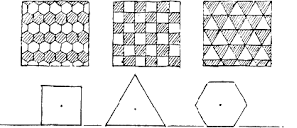
\includegraphics[width=\linewidth]{figuras/faradaysketcha.png}
                \caption{}
%                \label{fig:gull}
        \end{subfigure}%
        \begin{subfigure}[b]{0.20\textwidth}
                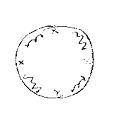
\includegraphics[width=\linewidth]{figuras/faradaysketchb.png}
                \caption{}
%                \label{fig:gull2}
        \end{subfigure}%
		\caption[Ilustraciones realizadas por Michael Faraday en su bitácora personal]{Ilustraciones realizadas por Michael Faraday en su bitácora personal \cite{Martin1832}. \textbf{(a)} Bocetos de patrones hexagonales, rectangulares y triangulares realizados por Faraday como posibles interpretaciones de la geometría de las crispaciones. \textbf{(b)} Diagrama de la vista superior realizada por Faraday de la distribución de crispaciones en un vaso de agua; ``x'' representa los lugares donde el de agua permanece inmóvil o las crispaciones son débiles, mientras que las líneas onduladas indican una superficie más agitada. \cite{Martin1832} } %sacado de Cavicchi
	\end{figure}
\end{center}

En 1954, Benjamin y Ursell desarrollaron una teoría lineal sobre la naturaleza subarmónica de la inestabilidad, realizando la verificación teórica directamente de la hidrodinámica \cite{Benjamin1954}. Sin embargo, el análisis de Benjamin y Ursell se basa en una aproximación de flujo potencial, la cual está restringida únicamente a fluidos no viscosos. Si la inestabilidad es generada en un líquido viscoso, una parte de la energía mecánica es disipada debido a esta viscosidad. Estos efectos generalmente se manejan agregando un amortiguamiento heurístico en la ecuación de Mathieu \cite{Landau1988}, que es proporcional a la viscosidad cinemática $\nu$. La inclusión de dicho término ha sido utilizado ampliamente en varios análisis lineales como los realizados por Müller \cite{Muller1993}; Kumar y Tuckerman \cite{Kumar1994}; Kumar \cite{Kumar1996} y Perlin y Schultz \cite{Perlin2000}. Sin embargo, esta aproximación ignora las capas límite viscosas a lo largo de las paredes del contenedor y por debajo de la superficie, donde se produce una disipación adicional. \medskip

La descripción matemática completa del problema involucra las ecuaciones de Navier-Stokes en un dominio con una superficie libre, donde las amplitudes de los modos normales se desacoplan y cumplen en primera aproximación de la ecuación de Mathieu, la cual es una ecuación diferencial ordinaria de segundo orden no autónoma. Un sistema no autónomo es un sistema de ecuaciones diferenciales ordinarias que depende explícitamente de la variable independiente. En este caso, la falta de autonomía está dada por el forzamiento externo que influye en los parámetros del fluido cuando se inicia el comportamiento oscilante. Benjamin y Ursell pudieron utilizar las propiedades de estabilidad conocidas de la ecuación de Mathieu para confirmar el punto de vista de Faraday y Rayleigh. Al tipo de inestabilidad presente en la ecuación de Mathieu se le llama \textit{Inestabilidad paramétrica}, y es conocida por estar presente en diversos sistemas como osciladores electrónicos, ondas de Langmuir en plasma y hasta en el comportamiento estocástico de un conjunto de precios. El experimento mas representativo de este fenómeno es el péndulo excitado paramétricamente. El cual consiste en un péndulo cuyo pivote es excitado verticalmente, lo que dará origen a la oscilación horizontal del péndulo con la mitad de la frecuencia de excitación para algunas amplitudes y frecuencias. En este caso, así como en el experimento de Faraday, la aceleración gravitacional efectiva es el parámetro externo propulsor. La ecuación de Mathieu debe su nombre al matemático francés E. L. Mathieu (1825-1890), quien en su trabajo original de 1868 muestra como resolver la ecuación de onda bidimensional para el movimiento de una membrana elíptica \cite{Mathieu1868}.\medskip

En las últimos 50 años se ha realizado un esfuerzo por ampliar el análisis de Benjamin y Ursell, a amplitudes finitas mediante la incorporación de no linealidades débiles, las cuales ha dado lugar a controversia. Por su parte, Dodge et al. \cite{Dodge1965}, Henstock y Sani \cite{Henstock1974} y Meron y Procaccia \cite{Meron1986} realizaron análisis para amplitudes finitas, resultado que son cuestionados por Miles \cite{Miles1984}. Ockendon y Ockendon \cite{Ockendon1973} extiende el análisis de Benjamin y Ursell a amplitudes pequeñas pero finitas, sin embargo, esto sin calcular explícitamente el parámetro de interacción que mide los efectos de inercia no lineales, siendo éstos los términos de tercer orden en las ecuaciones de movimiento. También determinan la estructura de bifurcación de las ecuaciones de evolución, incluyendo los efectos cualitativos del amortiguamiento lineal. Miles \cite{Miles1984}, por su parte, calcula el parámetro de interacción e incorpora el  amortiguamiento lineal. Gu et al. \cite{Gu1988} calculan el parámetro de interacción para un cilindro rectangular. Virnig et al. \cite{Virnig1988} pudieron medir las amplitudes de ondas en estado estacionario en grandes cilindros rectangulares en los que los efectos viscosos y capilares son pequeños, obteniendo resultados que coinciden razonablemente con los cálculos de Gu et al. \cite{Gu1988}. Con el creciente interés en la dinámica no lineal y el caos temporal, el experimento de Faraday ha ganado un interés más amplio. Keolian et al. \cite{Keolian1981} observó un estado caótico en un contenedor circular fuertemente impulsado.  Gollub y Meyer \cite{Gollub1983} estudiaron la transición al caos de un modo de oscilación único en una celda circular. Ciliberto y Gollub \cite{Ciliberto1984, Ciliberto1985} mostraron cómo los efectos de dos modos superpuestos puede conducir al caos. Simonelli y Gollub \cite{Simonelli1989} estudiaron las interacciones de dos modos casi degenerados por simetría. \medskip %lo de Dodge fue de Miles Single-modes

Otros estudios teóricos sobre la inestabilidad de Faraday han sido realizados por Miles \cite{Miles1984, Miles1993}, Miles y Henderson \cite{Miles1990}, Bechhoefer y Johnson \cite{Bechhoefer1996}, Müller et al. \cite{Muller1997}, Müller \cite{Muller1998a}, Mancebo y Vega \cite{Mancebo2002}, Huepe et al. \cite{Huepe2006}, y adicionalmente algunos estudios experimentales desarrollados por Douady \cite{Douady1990}, Edwards y Fauve \cite{Edwards1994}, Bechhoefer et al. \cite{Bechhoefer1995}, Kityk et al. \cite{Kityk2002}, Westra et al. \cite{Westra2003}, Residori et al. \cite{Residori2007}, Nguyem y Caps \cite{NguyemThuLam2011} para la formación de patrones. A partir de una elección adecuada de los parámetros experimentales, se pueden observar varios patrones distintos, que consisten en un conjunto de figuras geométricas ordenadas como rayas, cuadrados, triángulos y hexágonos. Kudrolli et al. \cite{Kudrolli1998} reportan patrones de superredes, mientras Arbell y Fineberg \cite{Arbell2000, Arbell2002} estructuras localizadas también se han observado utilizando forzamientos de dos frecuencias. Comprender los tipos de patrones que se forman es un desafío. El umbral de inestabilidad y los patrones observados dependen de la viscosidad y la tensión superficial del fluido, la aceleración adimensional de foramiento $\Gamma$, la forma y tamaño del recipiente. Además, las fluctuaciones en la frecuencia y amplitud de la fuerza impulsora pueden llevar a un patrón existente a un estado mixto con una fracción de caos espacio-temporal \cite{Kudrolli1996}.\medskip

En el límite de débil disipación, la comprensión de los resultados de los experimentos clásicos de Faraday se ha realizado basados en análisis lineales (Müller 1998) para un volumen de liquido espacialmente infinito. Además, los mecanismos de selección de patrones se han investigado utilizando las herramientas de simetría y teoría de la bifurcación \cite{Silber2000, Skeldon2007}. También han comenzado a aparecer simulaciones numéricas que implican la solución de las ecuaciones de Navier-Stokes acopladas a un método de seguimiento frontal para el tratamiento de la superficie libre, estas asumiendo que la superficie del líquido es perfectamente plana en las parades donde se aplican condiciones límite no deslizantes \cite{Perinet2009, Kahouadji2015}. Mas simulaciones numéricas han sido realizadas por otros autores como lo son las de Louis \cite{Louis2011} y Kentaro et al. \cite{Takagi2011, Takagi2015} Sin embargo, estas no dan cuenta del realismo de los  experimentos donde la dinámica del menisco es importante \cite{Douady1990}. En particular, para recipientes de pequeño tamaño existe un fuerte acoplamiento entre las ondas capilares generadas por el menisco y las ondas de Faraday \cite{NguyemThuLam2011}. Por otra parte, han surgido variantes particulares como la simulación realizada por Ebo Adou et al. en la cual una gota es sujeta a una fuerza externa periódica presentado inestabilidades de Faraday en su superficie.\medskip 

Mientras que los experimentos clásicos de patrones de onda de Faraday se refieren a contenedores individuales de diversos tamaños y formas, Delon et al. \cite{Delon2010} observaron la formación de patrones regulares en el caso en que la interfaz líquido-aire se dividió en una red de celdas cuadradas. Se ha encontrado que este tipo de experimentos tiene aplicaciones potenciales para la detección y ubicación de líquidos en las  cavidades internas de las estructuras tipo panal empleadas en construcciones mecánicas y aeronáuticas. La característica dinámica de los patrones de onda que surgen en los arreglos de celdas también ayuda a comprender el ensamblaje de los esferoides celulares en la bioingeniería para la construcción tridimensional de tejidos y organoides \cite{Chen2015}. De esta manera, las funciones de onda correspondientes pueden predecir patrones de ensamblaje de esferoides celulares de diferentes modos simétricos. Particularmente, nuestra atención se centra en el empleo de ondas de Faraday para la atomización ultrasónica de líquidos. La técnica de atomización ultrasónica tiene como ventaja sobre las técnicas de atomización convencionales que con este metodo se puede tener control sobre el tamaño de partícula y la densidad de la niebla. Los primeros trabajos sobre el empleo de la inestabilidad de Faraday para formación de micro gotas o la atomización ultrasónica datan de 1962, siendo este fenómeno fue descrito por primera vez por Wood y Loomis \cite{Wood1927} como un medio práctico para producir aerosoles utilizando frecuencias iguales o superiores a 20 kHz. Desde entonces, los dispositivos de baja frecuencia (20 {100 kHz) y alta frecuencia (0.1 {5 MHz) han evolucionado. Los primeros y más comúnmente usados son los cristales piezoeléctricos que impulsan un transductor de metal sobre el cual se coloca el líquido a ser atomizado. El funcionamiento y eficiencia básica de tales dispositivos han sido estudiadas experimentalmente por Lang \cite{Lano1962}, Pohlman y Stamm \cite{Pohlman1965}, Lierke y Griesshammer \cite{Lierke1967}, Topp \cite{Topp1973} (1973) y Sindayihebura et al. \cite{Sindayihebura1997}.\medskip 

Los estudios analíticos de Lang \cite{Lano1962}, Peskin y Raco \cite{Peskin1963} y Sindayihebura y Bolle \cite{Sindayihebura1997} se basan en el supuesto de que las gotas se forman en las crestas de las ondas capilares estacionarias presentes sobre la superficie de la película líquida. Yule y Al-Suleimani \cite{Yule2000} presentaron un estudio teórico para la expulsión aparentemente aleatoria de gotas de una celda de onda, aunque el modelo en sí es determinista; y Tsai et al. presentan una teoría lineal sobre la inestabilidad temporal de las ondas de Faraday para la eyección de microgotas monodispersas basada en la conservación de masa y las ecuaciones linealizadas de Navier-Stokes. Las investigaciones experimentales apuntan a comprender las características que dominan el proceso de atomización ultrasónica, donde analizan la distribución del tamaño de las gotas, velocidad de salida de las gotas o velocidad de atomización \cite{Barreras2002} \cite{Donnelly2004} y el efecto de las propiedades del los fluidos \cite{Avvaru2006, Ajay2013}. Las aplicaciones de la atomización ultrasónica empleando inestabilidades de Faraday son muy diversas. A la fecha, las investigaciones van dirigidas al rediseño de las boquillas de atomización ultrsónica para la maximización del caudal \cite{Dobre2002}, el estudio de los efectos de la aceleración a la cual es sometida la película de líquido y la ruptura de esta \cite{Cartellier2006}, y la validación de nuevo inyectores que combina los efectos de corte con el principio de atomización ultrasónica \cite{Boukra2009}.\medskip

%----------------------------------------------------------------

En esta tesis presentamos un estudio ... \textit{\textbf{Aquí iría una breve descripción del contenido de la tesis por capítulos. No mas de media cuartilla.}}
